\begin{table}[!tbp]
\centering
\caption{PXMem against KaPoCE on the twelve held-out SNAP graphs,
$T=\SI{600}{s}$ (primary budget), ten seeds per graph.  W/T/L: runs in
which PXMem is better, equal, worse.  median, HL: median and Hodges--Lehmann
estimate of $(\cost_{\mathrm{PXMem}}-\cost_{\mathrm{KaPoCE}})/
\cost_{\mathrm{KaPoCE}}$ in percent, negative when PXMem is better, with the
exact $95\%$ confidence interval; $p$: exact sign test over the seeds;
$p_{\mathrm{Holm}}$: Holm-adjusted over the twelve graphs.  Last row: the
pre-registered tests over the twelve graph medians.}
\label{tab:h2h-600}
\footnotesize
\setlength{\tabcolsep}{4pt}
\pending{}

\end{table}

\begin{table}[!tbp]
\centering
\caption{As Table~\ref{tab:h2h-600}, $T=\SI{150}{s}$.}
\label{tab:h2h-150}
\footnotesize
\setlength{\tabcolsep}{4pt}
\begin{tabular}{lrcrlrr}
\toprule
graph & runs & W/T/L & median (\%) & HL (\%) [95\% CI] & $p$ & $p_{\mathrm{Holm}}$ \\
\midrule
\texttt{email-Eu-core} & 6 & 0/5/1 & $+0.000$ & $+0.000$ [$+0.000$, $+0.008$] & 1.000 & 1.000 \\
\texttt{facebook} & 6 & 0/6/0 & $+0.000$ & $+0.000$ [$+0.000$, $+0.000$] & 1.000 & 1.000 \\
\texttt{wiki-Vote} & 6 & 5/0/1 & $-0.008$ & $-0.007$ [$-0.016$, $+0.026$] & 0.219 & 1.000 \\
\texttt{cit-HepTh} & 5 & 4/0/1 & $-0.009$ & -- & 0.375 & 1.000 \\
\texttt{cit-HepPh} & 6 & 3/0/3 & $-0.000$ & $-0.000$ [$-0.021$, $+0.039$] & 1.000 & 1.000 \\
\texttt{p2p-Gnutella31} & 6 & 0/4/2 & $+0.000$ & $+0.000$ [$+0.000$, $+0.001$] & 0.500 & 1.000 \\
\texttt{soc-Slashdot0902} & 6 & 0/0/6 & $+0.006$ & $+0.007$ [$+0.004$, $+0.010$] & 0.031 & 0.375 \\
\texttt{loc-Gowalla} & 5 & 0/0/5 & $+0.008$ & -- & 0.062 & 0.688 \\
\texttt{email-EuAll} & 5 & 5/0/0 & $-0.011$ & -- & 0.062 & 0.688 \\
\texttt{amazon0302} & 5 & 0/0/5 & $+0.008$ & -- & 0.062 & 0.688 \\
\texttt{web-NotreDame} & 5 & 0/0/5 & $+0.022$ & -- & 0.062 & 0.688 \\
\texttt{roadNet-PA} & 4 & 0/0/4 & $+0.507$ & -- & 0.125 & 0.875 \\
\midrule
\multicolumn{7}{l}{graph medians: 4 better, 3 equal, 5 worse; Wilcoxon $p=0.652$, sign test $p=1.000$} \\
\bottomrule
\end{tabular}

\end{table}

\begin{table}[!tbp]
\centering
\caption{As Table~\ref{tab:h2h-600}, $T=\SI{60}{s}$.}
\label{tab:h2h-60}
\footnotesize
\setlength{\tabcolsep}{4pt}
\pending{}

\end{table}

\paragraph{Primary budget.}  At \SI{600}{s} (Table~\ref{tab:h2h-600},
\numHHSixRuns{} paired runs) the graph medians favour PXMem on
\numHHSixBetter{} graphs and KaPoCE on \numHHSixWorse{}, with
\numHHSixEqual{} ties.  Neither pre-registered test rejects equality of the
two solvers (Wilcoxon $p=\numHHSixWilcoxon$, sign test
$p=\numHHSixSign$).  After Holm's correction PXMem is better on
\texttt{loc-Gowalla} and KaPoCE on \texttt{amazon0302} and
\texttt{roadNet-PA}; PXMem wins nine of ten seeds on \texttt{wiki-Vote},
\texttt{cit-HepTh} and \texttt{cit-HepPh}, which is not significant after the
correction.  All differences are small: the largest graph median is
\numHHSixMaxAbs{}, and on the held-out graphs with a certificate the
certified gap of the best solution is at least \numSnapGapMinHeld{}
(Table~\ref{tab:snap-bounds}).  The certificates therefore cannot separate
the two solvers, and neither solver is shown to be near-optimal on these
graphs beyond what Table~\ref{tab:snap-bounds} certifies.  KaPoCE returned a
valid solution in every run (\numHHSixForfeitK{} forfeits).  Scoring PXMem at
$T$ instead of at KaPoCE's elapsed time gives \numHHSixAtTBetter{} better and
\numHHSixAtTWorse{} worse graph medians (Wilcoxon $p=\numHHSixAtTWilcoxon$).
Many per-seed differences are zero or tied on some graphs
(\texttt{email-Eu-core}, \texttt{facebook}, \texttt{p2p-Gnutella31}); there
the Hodges--Lehmann interval degenerates and its coverage is not exact, and
zero graph medians are dropped from the Wilcoxon test, which the analysis
plan did not specify.  We do not claim that the two solvers are
equivalent: the study was not designed as an equivalence test.

\paragraph{Shorter budgets.}  KaPoCE did not stop by itself and was
terminated by SIGTERM in \numHHSixSigterm{}, \numHHOneFiftySigterm{} and
\numHHSixtySigterm{} of the 120 runs at \SI{600}{s}, \SI{150}{s} and
\SI{60}{s}; it then writes its best solution, which can take some seconds,
while PXMem is scored at KaPoCE's elapsed time.  This favours KaPoCE.  At
\SI{150}{s} (Table~\ref{tab:h2h-150}) the picture is similar (\numHHOneFiftyBetter{} better, \numHHOneFiftyEqual{}
equal, \numHHOneFiftyWorse{} worse; Wilcoxon $p=\numHHOneFiftyWilcoxon$),
with larger losses of PXMem on the largest graphs, up to
\numHHOneFiftyMaxAbs{} on \texttt{roadNet-PA}.  At \SI{60}{s}
(Table~\ref{tab:h2h-60}) KaPoCE is better on \numHHSixtyWorse{} of the
\numHHSixtyGraphs{} graph medians (Wilcoxon $p=\numHHSixtyWilcoxon$).  PXMem is
a population method, and a short budget leaves few recombinations on graphs
with $10^5$ vertices or more; we did not analyse this further.  PXMem is thus
not a replacement for KaPoCE at short budgets, and at the primary budget the
two are not distinguishable by our tests.

\paragraph{PACE heuristic track.}  On the 200 instances of the PACE~2021
heuristic track, one run per instance at \SI{600}{s} under the same protocol,
the instance is the unit.  The \numPDn{} instances that coincide with
development graphs are reported separately (Table~\ref{tab:pace-heur}).  On
the other \numPHn{} instances PXMem is better on \numPHBetter{}, equal on
\numPHEqual{} and worse on \numPHWorse{} (Wilcoxon $p=\numPHWilcoxon$, sign
test $p=\numPHSign$); KaPoCE returned no valid solution on
\numPHKapoceInvalid{} instances, which count as PXMem wins as in PACE.
The counts hide the sizes of the differences: summed over the \numPHn{}
instances the costs favour KaPoCE by 5185, and the eleven instances with
$10^5$ vertices or more contribute 5344 of this (PXMem better on six of
them, worse on five).
PXMem records its first solution only after its initialisation; on
\numPHNoSolution{} small instance KaPoCE stopped before that, and it
counts as a KaPoCE win under the protocol.
Figure~\ref{fig:profile} shows the performance profile.

\begin{table}[!tbp]
\centering
\caption{PACE~2021 heuristic track, $T=\SI{600}{s}$, one run per instance:
PXMem against KaPoCE by instance size.  W/T/L: instances on which PXMem is
better, equal, worse; $\sum$: total difference of the costs; median: of the
relative differences in percent.}
\label{tab:pace-heur}
\footnotesize
\begin{tabular}{l}
\pending{} (54 of 200 runs done)
\end{tabular}

\end{table}

\begin{figure}[!tbp]
\centering
\IfFileExists{figures/profile_pace_heur.pdf}{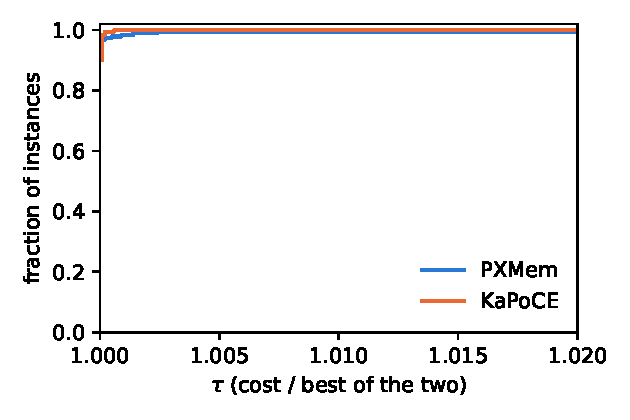
\includegraphics[width=0.6\textwidth]{figures/profile_pace_heur.pdf}}{\pending{}}
\caption{Performance profile~\cite{DolanM02profiles} on the PACE heuristic
track without the development twins: fraction of instances on which a
solver's cost is within a factor $\tau$ of the better of the two.}
\label{fig:profile}
\end{figure}
